\chapter{Priprava na 11. laboratorijske vaje}
\section{Realizacija končnih avtomatov s pomnilnimi celicami (Mealyjev avtomat)}

Obnašanje Moorovega avtomata je že v osnovi sinhrono. Stanje avtomata se v odvisnosti od vhodne črke spremeni le ob urini fronti. Ker je izhodna črka neposredno odvisna le od njegovega stanja, se ta sinhrono spremeni ob spremembi stanja avtomata.\\

%Za razliko od Moorovega avtomata je pri Mealyjevemu avtomatu izhodna črka neposredno odvisna od stanja avtomata in vhodne črke. To pomeni, da se v primeru sprembe vhodne črke, izhodna črka lahko spremeni asinhrono (spremeni se v trenutku spremembe vhodne črke in ne le ob urini fronti oziroma spremembi stanja avtomata). Tako obnašanje ni dovoljeno in zahteva eksplicitno sinhronizacijo izhodne črke. To najenostavneje dosežemo tako, da izhodno vezje (realizacijo izhodne funkcije) vežemo na vhode D pomnilnih celic (pri realizaciji Mealyjevega avtomata z $n$ izhodnimi črkami torej potrebujemo še $\left\lceil \log_2(n)\right\rceil$ dodatnih D pomnilnih celic). S tem dosežemo, da se izhodna črka spremeni ob urini fronti, torej sinhrono s spremembo stanja avtomata.

Za razliko od Moorovega avtomata je pri Mealyjevem avtomatu izhodna črka neposredno odvisna od stanja avtomata in vhodnih spremenljivk. To pomeni, da se v primeru spremembe vhodne spremenljivke, izhodna črka lahko spremeni asinhrono (spremeni se v trenutku spremembe vhodne spremenljivke in ne le ob urini fronti oziroma spremembi stanja avtomata). Tako obnašanje ni dovoljeno in zahteva eksplicitno sinhronizacijo izhodne črke. To najenostavneje dosežemo tako, da izhodno vezje (realizacijo izhodne funkcije) vežemo na vhode D pomnilnih celic (pri realizaciji Mealyjevega avtomata z $n$ izhodnimi črkami torej potrebujemo še $\left\lceil \log_2(n)\right\rceil$ dodatnih D pomnilnih celic). S tem dosežemo, da se izhodna črka spremeni ob urini fronti, torej sinhrono s spremembo stanja avtomata.

Realizacija Mealyjevega avtomata je zelo podobna realizaciji Moorovega avtomata. Ponazorili jo bomo z zgledom, ki sledi.

\bigskip

\begin{zgled}

Realiziraj Mealyjev avtomat, ki je podan s tabelo prehajanja stanj. Za realizacijo notranjih stanj imaš na voljo T pomnilne celice, za generiranje izhodne črke pa D pomnilne celice. 

\begin{center}
\begin{tabular}{c|ccc}
 & $S_1$ & $S_2$ & $S_3$\\
\hline
$x_1$ & $S_2 / z_1$ & $S_2 / z_2$ & $S_1 / z_1$\\
$x_2$ & $S_1 / z_2$ & $S_3 / z_1$ & $S_3/ z_2$ \\
\end{tabular}
\end{center}

\end{zgled}

\begin{resitev}

Postopek je sledeč:

\begin{enumerate} 

\item Zapišemo kodirne tabele, ki določijo kodiranje vhodne abecede, notranje abecede in izhodne abecede. Za zapis vseh črk vhodne abecede je dovolj 1 vhodna spremenljivka ($x$); prav tako je za zapis vseh črk izhodne abecede dovolj 1 izhodna spremenljivka ($y$). Ker imamo tri notranja stanja avtomata, za njegovo realizacijo potrebujemo 2 pomnilni celici T z notranjimi stanji $q_1$ in $q_2$. Kodirne tabele so torej

\begin{table}[ht]
\begin{center}
\begin{tabular}{ccc}
	\begin{tabular}{c|c}
	 & $x$ \\ 
		\hline
		$x_1$ & $0$\\
		$x_2$ & $1$\\
	\end{tabular}
	&
	\begin{tabular}{c|cc}
		 & $q_1$ & $q_2$ \\ 
		\hline
		$S_1$ & $0$ & $0$ \\
		$S_2$ & $0$ & $1$\\
		$S_3$ & $1$ & $0$\\
	\end{tabular}
	&
	\begin{tabular}{c|c}
		 & $y$ \\ 
		\hline
		$z_1$ & $0$\\
		$z_2$ & $1$\\
	\end{tabular}
\end{tabular}
\end{center}
\end{table}

\bigskip

\item Na podlagi kodirnih tabel in podanega diagrama prehajanja stanj lahko zapišemo pravilnostno tabelo avtomata. Pri tem na levi strani tabele nastopajo spremenljivke, ki določajo trenutno notranje stanje avtomata ($q_1$ in $q_2$) in vhodno črko ($x$), na desni pa spremenljivke, ki določajo notranje stanje  ($D^1q_1$ in $D^1q_2$) in izhodno črko ($D^1y$) v naslednjem časovnem koraku. Vrednosti izhodne črke določamo na podlagi prehodov med stanji.

\begin{center}
\begin{tabular}{ccc|ccc}
 $q_1$ & $q_2$ & $x$ & $D^1 q_1$ & $D^1 q_2$ & $D^1y$\\
  \hline
 0 & 0 & 0 & 0 & 1 & 0\\		 
 0 & 0 & 1 & 0 & 0 & 1\\		 
 0 & 1 & 0 & 0 & 1 & 1\\		 
 0 & 1 & 1 & 1 & 0 & 0\\		 
 1 & 0 & 0 & 0 & 0 & 0\\		 
 1 & 0 & 1 & 1 & 0 & 1\\		 
 1 & 1 & 0 & ? & ? & ?\\		 
 1 & 1 & 1 & ? & ? & ?\\		 
\end{tabular}
\bigskip
\bigskip
\end{center}

\item Na podlagi prehodov med spremenljivkami $q_1$ in $D^1q_1$ ter $q_2$ in $D^1q_2$ in vzbujevalne tabele za T pomnilno celico, lahko določimo vrednosti, ki morajo biti na vhodih T pomnilnih celic ($t_1$ in $t_2$). Poleg tega določimo tudi vhode v D pomnilno celico, ki služi sinhronizaciji izhodne črke.

\begin{center}
\begin{tabular}{ccc|ccc|cc|c}
 $q_1$ & $q_2$ & $x$ & $D^1 q_1$ & $D^1 q_2$ & $D^1y$ & $t_1$ & $t_2$ & $d$\\
  \hline
 0 & 0 & 0 & 0 & 1 & 0 & 0 & 1 & 0\\		 
 0 & 0 & 1 & 0 & 0 & 1 & 0 & 0 & 1\\		 
 0 & 1 & 0 & 0 & 1 & 1 & 0 & 0 & 1\\		 
 0 & 1 & 1 & 1 & 0 & 0 & 1 & 1 & 0\\		 
 1 & 0 & 0 & 0 & 0 & 0 & 1 & 0 & 0\\		 
 1 & 0 & 1 & 1 & 0 & 1 & 0 & 0 & 1\\		 
 1 & 1 & 0 & ? & ? & ? & ? & ? & ?\\		 
 1 & 1 & 1 & ? & ? & ? & ? & ? & ?\\		 
\end{tabular}
\bigskip
\end{center}

\item Na podlagi pravilnostne tabele lahko s pomočjo Veitchevega diagrama izpišemo funkciji, ki nastopata na vhodih T pomnilnih celic in D pomnilne celice avtomata:


\begin{figure}[!ht]
\begin{center}
\begin{tabular}{cc}

\includegraphics{veitch_mealy_t_1.eps} &

\includegraphics{veitch_mealy_t_2.eps} \\
$t_1 = q_1 \ol x \vee q_2 x$ & $t_2 = x q_2 \vee \ol x_{\ } \ol q_1 \ol q_2$\\
\end{tabular}
\end{center}
\end{figure}

\begin{figure}[!ht]
\begin{center}
\begin{tabular}{c}

\includegraphics{veitch_mealy_y.eps} \\
$d = x \ol q_2 \vee \ol x q_2 = x \nabla q_2$\\
\end{tabular}
\end{center}
\end{figure}

Pri tem izhod iz D pomnilne celice realizira izhodno črko avtomata. Po definiciji velja, da je izhodna črka Mealyjevega avtomata določena s trenutnim stanjem in vhodno črko avtomata. Velja torej, da za realizacijo funkcije izhodne črke (funkcija, ki vstopa na vhodu D pomnilne celice) v splošnem potrebujemo tako spremenljivke, ki določajo trenutno stanje avtomata kot tudi spremenljivke, ki določajo vhodne črke avtomata.

\end{enumerate}

\bigskip

Realizacijo avtomata v Logisimu prikazujejo slike \ref{fig:logisim}, \ref{fig:logisim_f}(a), \ref{fig:logisim_f}(b) in \ref{fig:logisim_f}(c).

\begin{figure}[ht]
\begin{center}
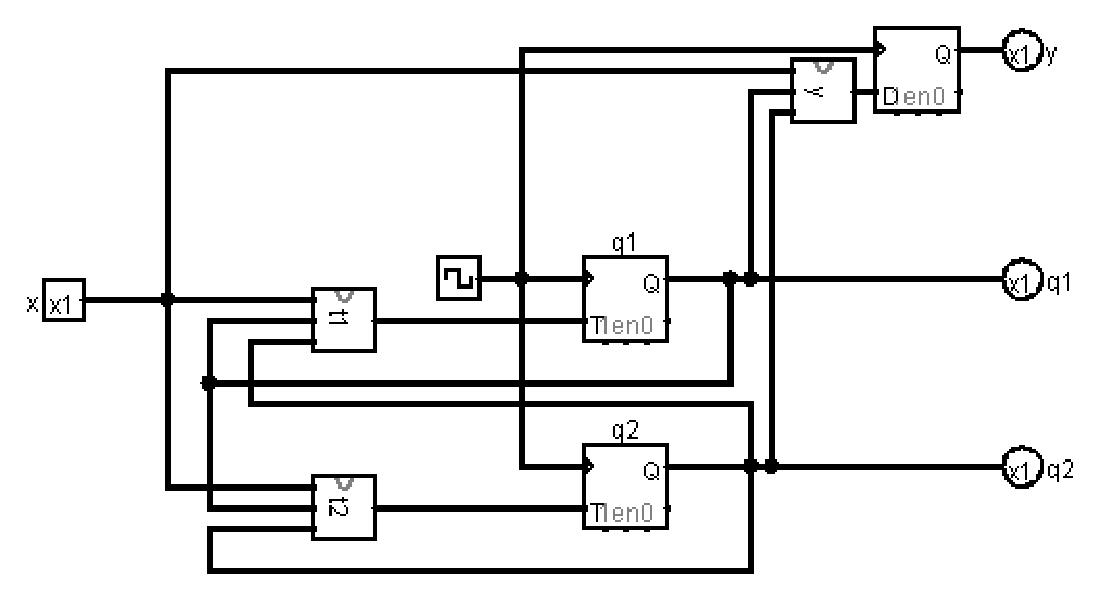
\includegraphics[width=0.5\linewidth]{mealy_logisim_sync.eps}
\end{center}
\caption{Realizacija avtomata v Logisimu. Zaradi preglednosti sta funkciji, ki vstopata v pomnilni celici T in izhodna funkcija realizirane v ločenih modulih (glej slike \ref{fig:logisim_f}(a), \ref{fig:logisim_f}(b) in \ref{fig:logisim_f}(c).}
\label{fig:logisim}
\end{figure}

\begin{figure}[!ht]
\begin{center}
\begin{tabular}{cc}
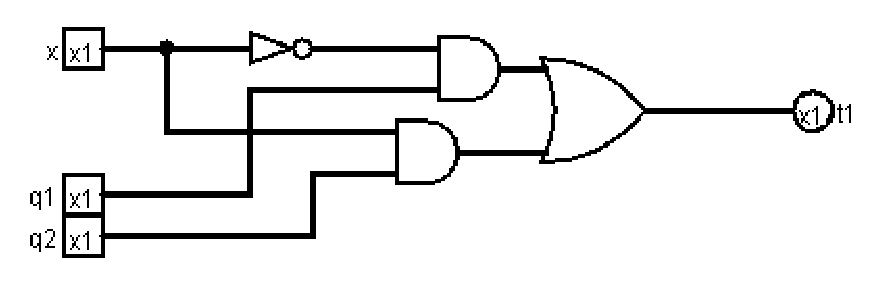
\includegraphics[width=0.47\linewidth]{mealy_logisim_t1.eps} &
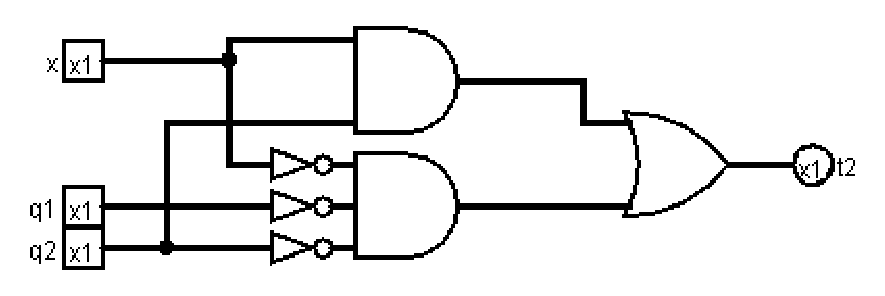
\includegraphics[width=0.47\linewidth]{mealy_logisim_t2.eps} \\
(a) & (b) \\
\end{tabular}

\bigskip

\begin{tabular}{c}
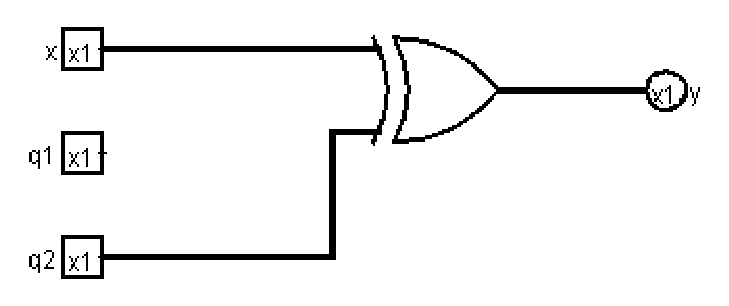
\includegraphics[width=0.37\linewidth]{mealy_logisim_y.eps}\\
(c) \\
\end{tabular}
\caption{Realizacija preklopne funkcije, ki vstopa v T pomnilno celico z vhodom $t_1$ (a), preklopne funkcije, ki vstopa v T pomnilno celico z vhodom $t_2$ (b) in izhodne funkcije avtomata (c).}
\label{fig:logisim_f}
\end{center}
\end{figure}

\end{resitev}

%
%\subsection*{Realizacija sinhronskega Mealyjevega avtomata}
%
%Izhodno črko bomo sinhronizirali tako, da jo bomo na izhod vezali preko pomnilnih celic. V primeru, da je izhodna abeceda sestavljena iz $n$ črk, bomo torej za realizacijo sinhronskega Mealyjevega avtomata potrebovali dodatnih $n$ pomnilnih celic. Zaradi enostavnosti bomo predpostavili, da imamo za potrebe sinhronizacije izhodnih črk vedno na voljo D pomnilne celice. 
%
%\begin{zgled}
%Realiziraj sinhronski Mealyjev avtomat iz Zgleda 1, pri čemer imaš za realizacijo notranjih stanj na voljo T pomnilne celice, za sinhronizacijo izhodov pa D pomnilne celice.
%
%\bigskip
%
%Pri realizaciji sinhronskega Mealyjevega avtomata lahko izhajamo iz asinhronskega, ki mu dodamo sinhronizacijo izhodnih črk. Ker imamo asinhronsko različico že realizirano (glej Zgled 1), gremo lahko neposredno na shemo sinhronske realizacije, ki jo prikazuje slika \ref{fig:logisim_sync}.
%
%\begin{figure}[ht]
%\begin{center}
%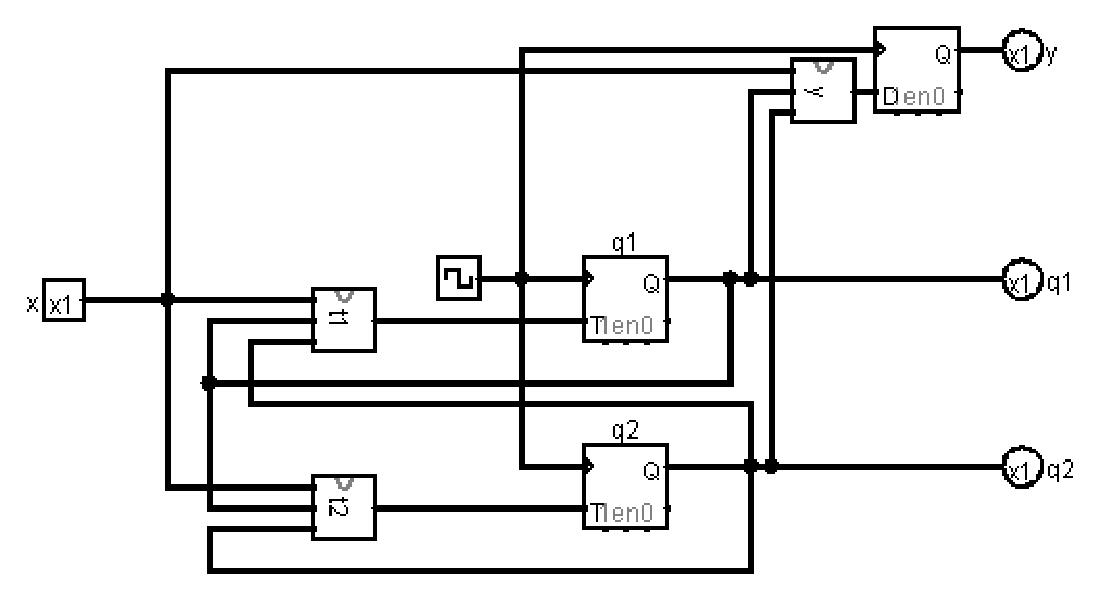
\includegraphics[width=0.5\linewidth]{mealy_logisim_sync.eps}
%\end{center}
%\caption{Realizacija sinhronskega Mealyjevega avtomata v Logisimu. Funkciji, ki vstopata v pomnilni celici T in izhodna funkcija so enake kot v Zgledu 1 (glej slike \ref{fig:logisim_f}(a), \ref{fig:logisim_f}(b) in \ref{fig:logisim_f}(c)). Edina razlika od asinhronske realizacije je D pomnilna celica pred izhodno spremenljivko y.}
%\label{fig:logisim_sync}
%\end{figure}
%
%\end{zgled}

